\documentclass[12pt]{article}
\usepackage[utf8]{inputenc}
\usepackage{geometry}
\usepackage[T1]{fontenc}
\usepackage{amsfonts}
\usepackage{afterpage}
\usepackage{graphicx}
\usepackage{float}
\usepackage{url}
\usepackage{hyperref}
\usepackage{bookmark}
\usepackage[sorting=none]{biblatex}
\usepackage{multirow}
\usepackage[table,xcdraw]{xcolor}
\usepackage{pgf}
\usepackage{xurl}
\usepackage{tabularray}
\usepackage{tabulary}
\usepackage{fancyhdr}
\usepackage[maxfloats=30,morefloats=12]{morefloats}
\usepackage{multicol}
\usepackage[dvipsnames]{xcolor}
\usepackage{awesomebox}
\usepackage{caption,subcaption} 
\usepackage{pgfornament}
\usepackage[export]{adjustbox}
\usepackage{tikzlings}
\usepackage{fontawesome5} 

\addbibresource{howto.bib} %Import the bibliography file
\fontfamily{put}\selectfont
\setlength{\columnsep}{40pt}
\setlength{\voffset}{0.5cm}
\setlength{\headsep}{40pt}
\setlength{\headheight}{34.06914pt} % Fix for fancyhdr error
\addtolength{\topmargin}{-22.06914pt} % Adjusted top margin as suggested by fancyhdr
\geometry{legalpaper, portrait, margin=2.3cm}

% Header and footer
\pagestyle{fancy}
\fancyhead[C]{
\includegraphics[width=0.05\textwidth]{images/escudo.png}}
\fancyhead[L]{\textbf{Tópicos II}\\ Universidad de Concepción}
\fancyhead[R]{\textbf{Florencia Fuentes}\\flofuentes2021@udec.cl}
\fancyfoot{}
% for adjust width environment
\usepackage[strict]{changepage}

% for formal definitions
\usepackage{framed}

%\definecolor{formalshade}{rgb}{0.95,0.95,1}
\definecolor{formalshade}{rgb}{.97, .88, .94}

\newenvironment{formal}{
  \def\FrameCommand{
    \hspace{1pt}
    {\color{White}\vrule width 2pt}
    {\color{Lavender}\vrule width 4pt}
    \colorbox{formalshade!40!white}
  }
  \MakeFramed{\advance\hsize-\width\FrameRestore}%
  \noindent\hspace{-4.55pt}% disable indenting first paragraph
  \begin{adjustwidth}{}{7pt}%
  \vspace{2pt}\vspace{2pt}
}
{\vspace{2pt}\end{adjustwidth}\endMakeFramed}

\renewcommand{\headrulewidth}{0.1pt}

\usepackage{tikz}

\usepackage{tcolorbox}
\tcbuselibrary{minted}
\newtcblisting{mybox}{colback=white,minted language=latex,listing side text,righthand width=.5\textwidth}
\usetikzlibrary{ducks}
\usepackage{tikzducks}

\definecolor{titlepagecolor}{cmyk}{0,.59,.25,.21}

\newcommand\titlepagedecoration{%
\begin{tikzpicture}[remember picture,overlay,shorten >= -10pt]

\coordinate (aux1) at ([yshift=-15pt]current page.north east);
\coordinate (aux2) at ([yshift=-410pt]current page.north east);
\coordinate (aux3) at ([xshift=-4.5cm]current page.north east);
\coordinate (aux4) at ([yshift=-150pt]current page.north east);

\begin{scope}[titlepagecolor!70,line width=12pt,rounded corners=12pt]
\draw
  (aux1) -- coordinate (a)
  ++(225:5) --
  ++(-45:5.1) coordinate (b);
\draw[shorten <= -10pt]
  (aux3) --
  (a) --
  (aux1);
\draw[opacity=0.6,titlepagecolor,shorten <= -10pt]
  (b) --
  ++(225:2.2) --
  ++(-45:2.2);
\end{scope}
\draw[titlepagecolor,line width=8pt,rounded corners=8pt,shorten <= -8pt]
  (aux4) --
  ++(225:0.8) --
  ++(-45:0.8);
\begin{scope}[titlepagecolor!70,line width=6pt,rounded corners=8pt]
\draw[shorten <= -10pt]
  (aux4) --
  ++(225:3) coordinate[pos=0.45] (c) --
  ++(-45:3.1);
\draw
  (aux4) --
  (c) --
  ++(135:2.5) --
  ++(45:2.5) --
  ++(-45:2.5) coordinate[pos=0.3] (d);   
\draw 
  (d) -- +(45:1);
\end{scope}
\end{tikzpicture}%
}

\DeclareFixedFont{\titlefont}{T1}{ppl}{b}{it}{0.5in}

\let\hrefWithoutArrow\href

\renewcommand{\href}[2]{\hrefWithoutArrow{#1}{\ifthenelse{\equal{#2}{}}{ }{#2 }\raisebox{.15ex}{\footnotesize \faExternalLink*}}}


\begin{document}
  % environment derived from framed.sty: see left bar environment definition
    \pagecolor{pink!40!white}\afterpage{\nopagecolor}
    %\maketitle

    \begin{titlepage}
        \centering

        
\includegraphics[width=0.2\textwidth,left]{images/escudo.png}

        \vspace*{5cm}

        {\Huge\bfseries
        
        Avance de Tesis
        \par}

        \vspace{0.2cm}

        {\raggedleft\Large\itshape `Optimización y caracterización \\ de Tapered Amplifiers' \qquad  \par}

        \vfill


        {\Large \bfseries Florencia Fuentes Jara \par} 

        
        \vspace{0.1cm}

        \mbox{\hrefWithoutArrow{mailto:flofuentes2021@udec.cl}{\color{magenta}{\footnotesize\faEnvelope[regular]}\hspace*{0.13cm}flofuentes2021@udec.cl}}%

        \vspace{1cm}

        {\large
        Universidad de Concepción\\
        Faculty of Physical and Mathematical Sciences\\
        Department of Physics
        \par}

        \titlepagedecoration
    \end{titlepage}

    \thispagestyle{fancy}
    \newpage
    % Table of Contents
    \tableofcontents
    \thispagestyle{fancy}

    \clearpage

    % Begin page numbers
    \fancyfoot[C]{\thepage}
    \pagenumbering{arabic}

    \section{Resumen}

    \section{Tapered Amplifier}
      \subsection{¿Qué es?}
      \begin{figure}[H] % FIXED: Added layout control identifier
        \centering
        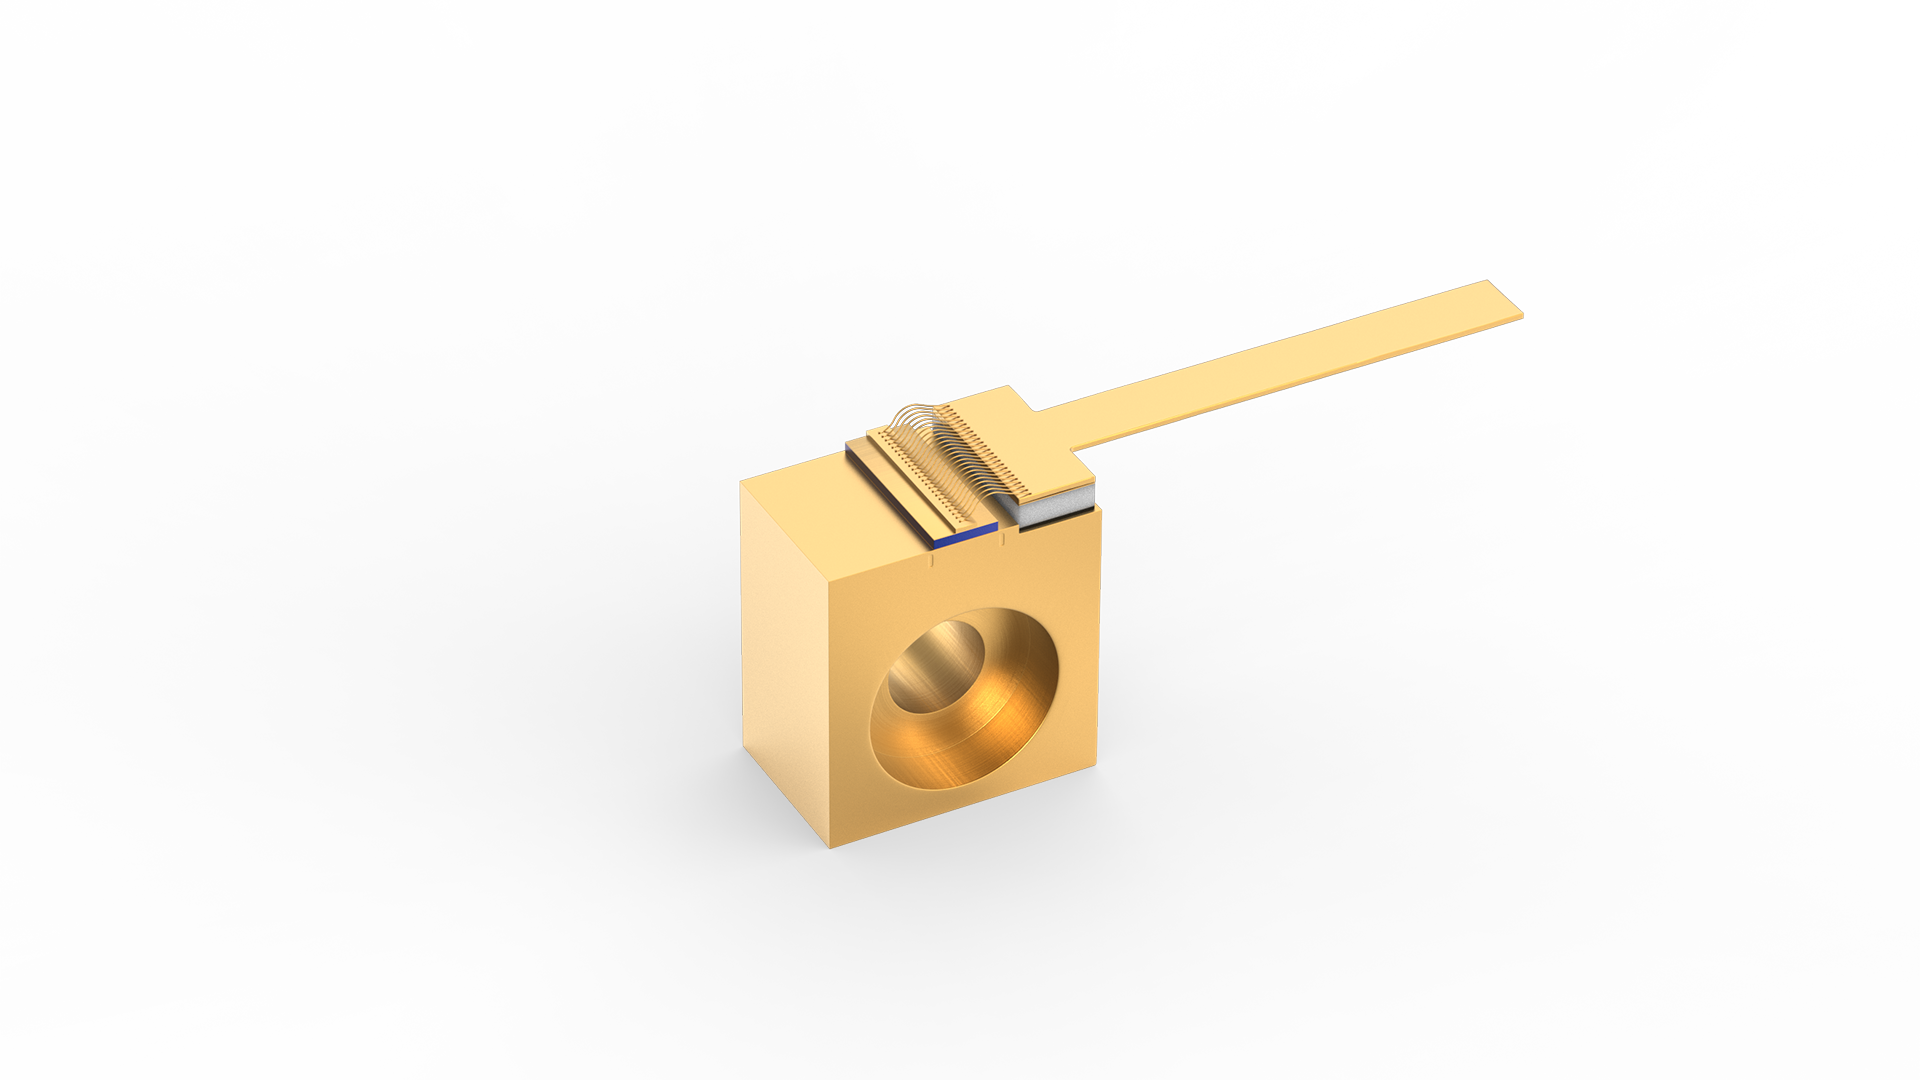
\includegraphics[width=0.6\textwidth]{Images/TA_img.png} % FIXED: Scaled width down to prevent page overflows
      \end{figure}

      \subsection{¿Cómo funciona?} % FIXED: Corrected spelling accent of "¿Cómo funciona?"

      \begin{formal}
      \ \textbf{Emisión estimulada espontánea (ASE)} % FIXED: Corrected spelling accent of "espontánea"
      \end{formal}


      \subsection{¿Para qué se utiliza?} % FIXED: Corrected spelling accent of "¿Para qué...?"
      \subsection{Control del TA}
        \subsubsection{Control de Temperatura}
        \subsubsection{Control de Corriente}
        \subsubsection{Circuito de Protección}
      \subsection{Medidas de Precaución}

    \section{MOPA Setup}
aaaaaaa
    \section{Simulaciones en LTspice}
    
    \begin{figure}[htbp]
      \centering
      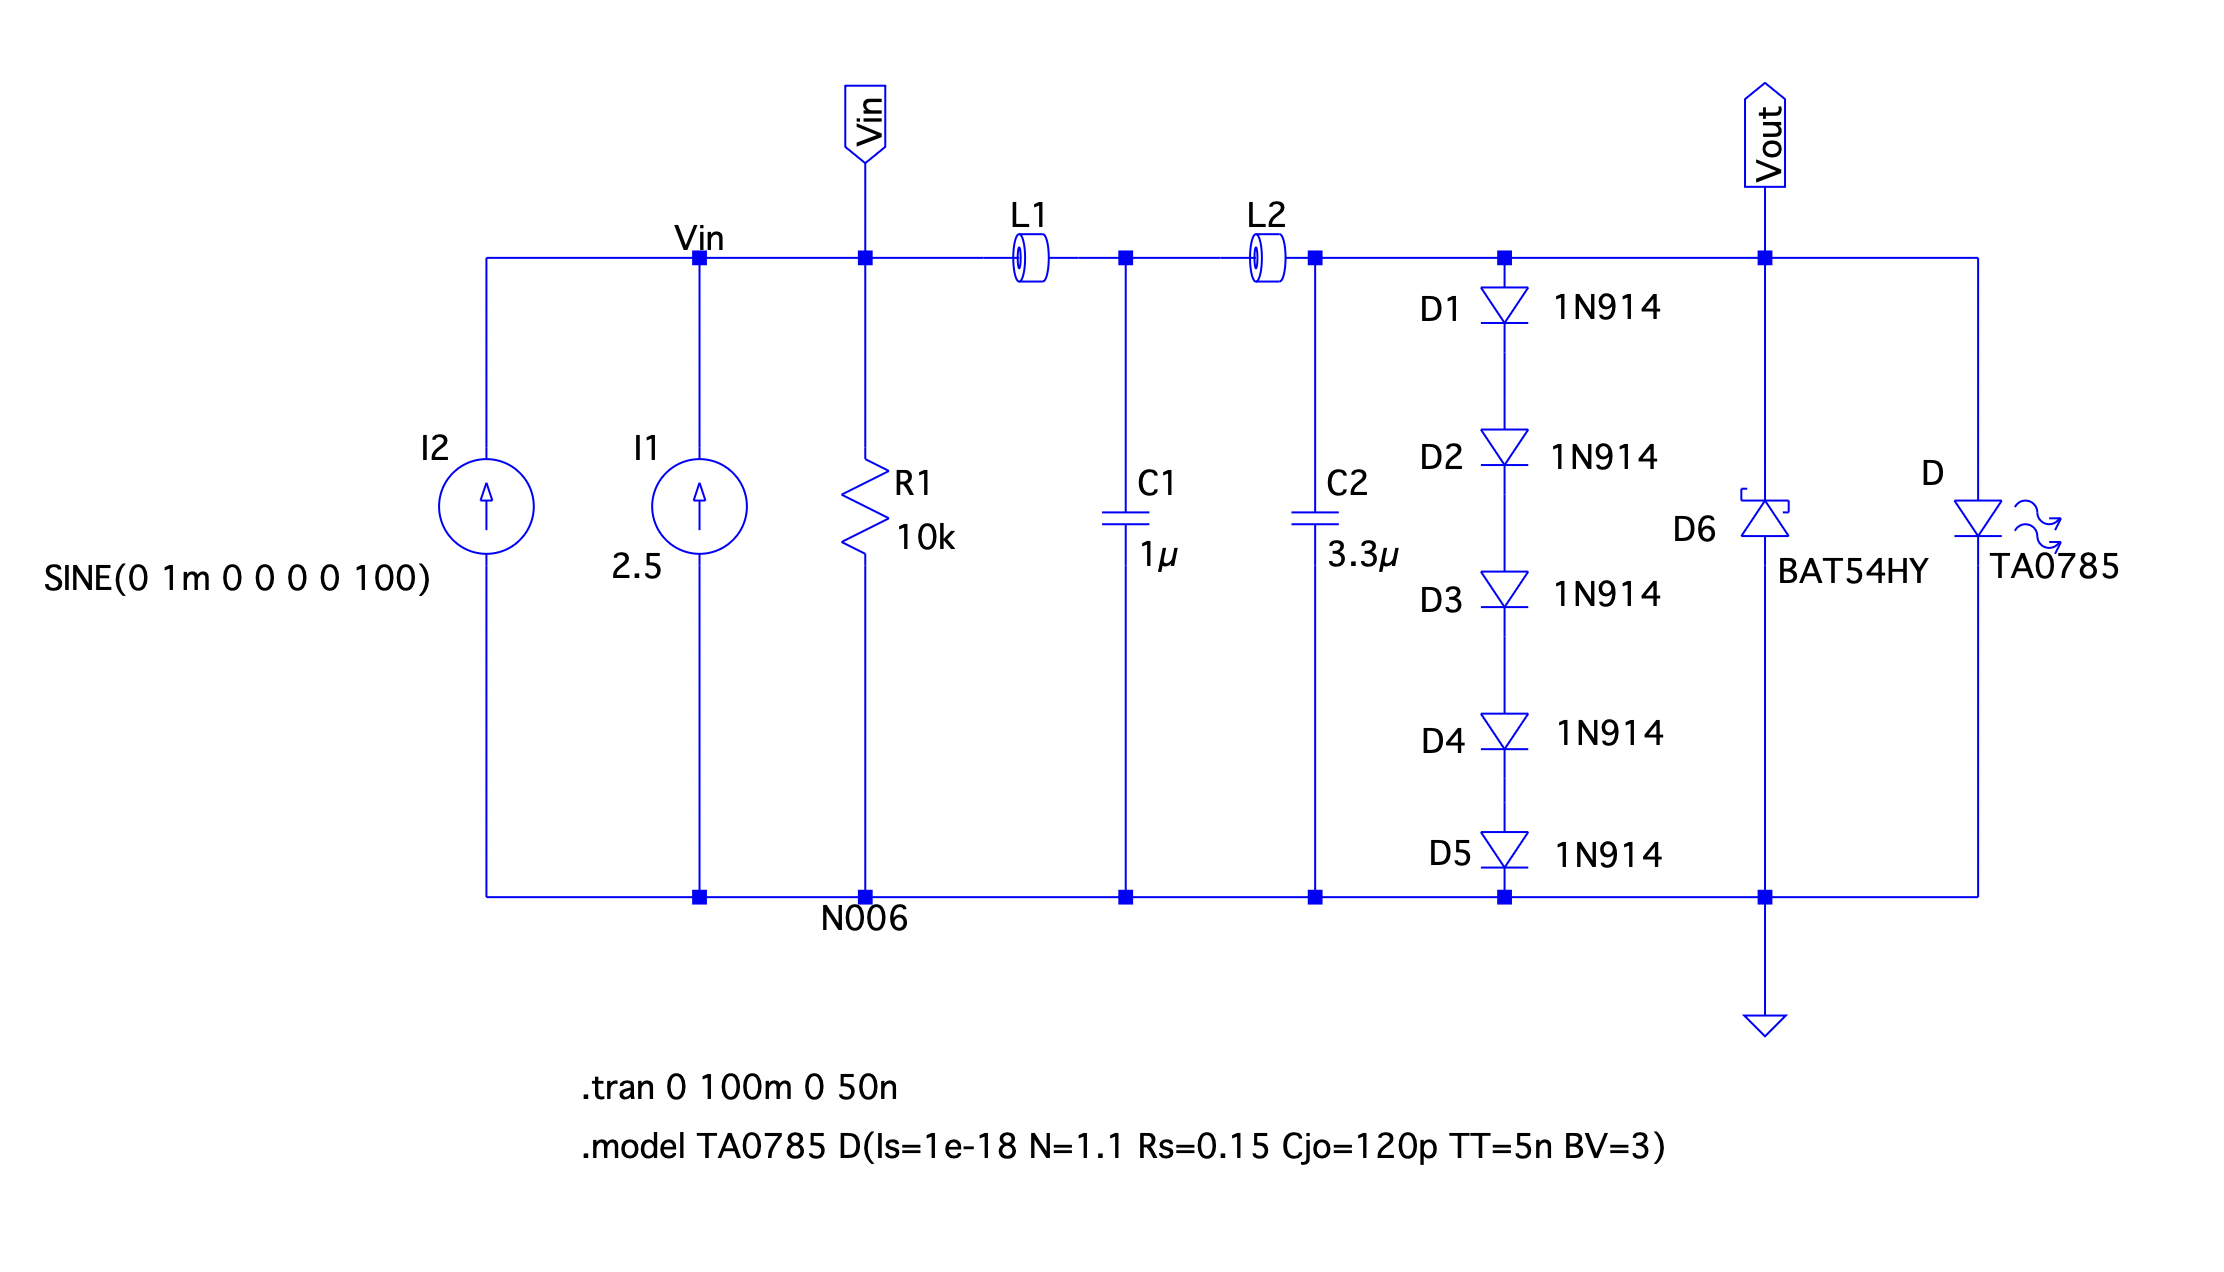
\includegraphics[width=0.8\linewidth]{Images/SC_TA.png} % FIXED: Trimmed down from \linewidth to save vertical space
      \caption{Simulación circuito de protección del TA}
      \label{fig:ta}
    \end{figure}
    % ===============================
    % REFERENCES SECTION
    % ===============================
    \section*{References}
     \addcontentsline{toc}{section}{References}
    % \printbibliography[heading=none]
    % \newpage
    % ===============================

    %\appendix\label{apx}

 \end{document}